\chapter{基于概念漂移检测的短文本数据流分类算法设计}

% \section{引言}                  
本文提出一种基于概念漂移检测的短文本数据流分类算法,用于对短文本数据流进行隐含主题的跟
踪。该方法采用集成学习,将时序的文本数据流进行分块,针对每个块训练一个基础SVM分类器,并根
新旧据块之间的语义距离判断是否发生概念漂移,结合分配给每个分类器的权重,动态地更新模型池中
的基分类器,使得模型池中始终保持恒定数量的分类器。对于新到来的未知标签的数据块,采用该集成
模型进行预测和分析,这就是本文提出的主题跟踪的算法基础。

% 接下来,本章会从问题定义开始,详细
% 介绍如何设计一个高效可用的集成模型。

\section{框架设计}

% 在这个部分,对于短文本数据流集成分类算法进行了形式化。
假定数据流由N个数据块组成,命名为$D = \{
D_1,  D_2,  …… , D_N \}$ ,每个数据块包含一些短文本,命名为$D_i = \{ d_1, d_2, …… , d_n \}$,
其中n表示第i个数据块的短文本数目。
通常,每个文档都能被表示成一个向量空间,命名为$d_j = \{ (v_x, v_y)  |  v_x \in R^M, v_y
\in Y\}$,其中$R^M$表示一个文档空间,Y表示该文档的标签,M表示维度。

为解决短文本数据流的稀疏性问题,本文使用Wikipedia作为外部语料库对短文本进行语义扩展,缓解
该问题,扩展后的数据块表示为$D_i^{'}=\{d_j^{'}\}_{j=1}^{|D_i|}$。然后使用BTM主题模型将扩展
后的数据块特征表示K维的主题分布,记作$D_i^{''}=\{d_j^{''}\}_{j=1}^{|D_i|}$。


最终,本文的目标是训练一个动态的集成模型$f : E_{\sum{D_i}}
\rightarrow Y$,将特征向量映射到标签上,以适应未知的短文本数据流并且发现短文本数据流中存在的概念漂移现象。

为了高效地处理短文本数据流分类问题,该方法的框架是由H个基分类器组合,构建一个集成分类模型 $E = \{ f_1, f_2, ……,f_h \}$。当新的数据块$d_j$来的时候,集成分类模型通过公式\ref{eq:1}赋予$d_j$一个类标签$y^*$。
  \begin{equation}
    \label{eq:predict}
    y^* = argmax_{y \in Y}P(y|d, E)     
  \end{equation}
    
其中后验概率$P(y|d, E)$是通过K个基分类模型进行加权平均所得,如公式\ref{eq:2}

\begin{equation}
  \label{eq:2}
  P(y|d, E) = \sum_{i=1}^{K}w_iP(y|d, f_i)
\end{equation}

% 在该方法中,每个文档d都可以被表示成一个个词特征向量。为了提取特征向量,需要识别短文本中所
% 包含的词。这涉及到接下来相关的两个重要技术,叫做特征表示和短文本扩展。

%通过统计得出,实验数据中短文本所占比
% 例达95,因此,我们仅用特征词特征空间来表示短文本,记作$ V_d = \{ T \}$。

图\ref{fig:shorttextclass}是整个算法的流程:

\begin{figure}[htb]
  \centering
  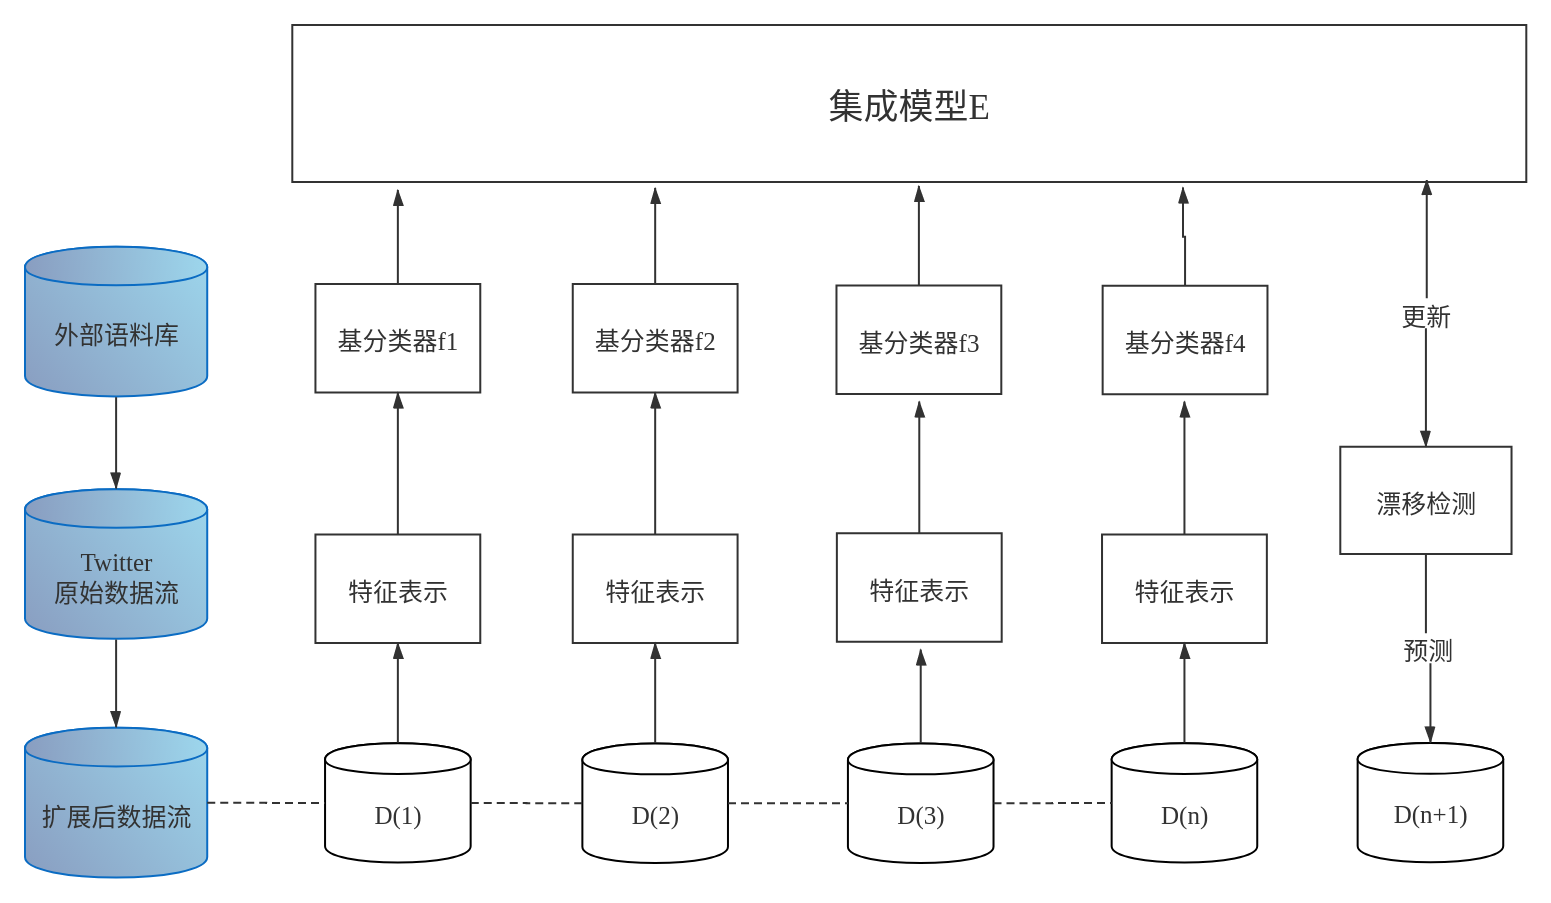
\includegraphics[width=1.0\textwidth]{shorttext}
  \caption{短文本数据流分类流程图}
  \label{fig:shorttextclass}
\end{figure}

% \section{数据预处理}

\section{数据采集与预处理}
本课题的实验数据来自Twitter,使用Twitter官方提供的“关键字搜索”API进行自动化采集。一共收集
了从2011年11月份到2013年1月份的5个类别的共约181万条数据。图\ref{tab:number}是每个类别的数量,图\ref{tab:exp}是数据实例。

\begin{table}[H]                                                                    \begin{singlespace}                                                          
    \centering\caption{每个类别的数量}\label{tab:number}
    \renewcommand{\arraystretch}{1.5} %控制行高
    \begin{tabular}{p{2.5cm}p{2cm}}\hline                                                        标签    
      & 数量 \\ \hline                                                
      \verb|arsenal| & 515017 \\                                                   
      \verb|blackfriday| & 137767 \\
      \verb|smartphone| & 401361 \\
      \verb|chelsea| & 647879 \\
     \verb|obama| & 112155 \\ \hline                                     
    \end{tabular}                                                                                       
  \end{singlespace}
\end{table}

\begin{table}[H]                                                                    \begin{singlespace}                                                          
    \centering\caption{类别实例}\label{tab:exp}
    \renewcommand{\arraystretch}{1.5} %控制行高
    \begin{tabular}{p{2.5cm}p{12.5cm}}\hline                                                        标签
      & 实例 \\ \hline                                                
      \verb|arsenal| & why arsenal fans always proud of their history, are they living in past? \\                                                   
      \verb|blackfriday| &  BeachBody's having Black Friday deals too! Check out these
                           great deals! http://t.co/NphfZ5Xu \\
      \verb|smartphone| & @MsEmeraldEyez ok got you posted up here: http://t.co/jzPIpstF feel special ur the 1st one :)            \\
      \verb|chelsea| &   @chelseaaaakay god fucking damnit Chelsea you don't get it.                                                                                \\
     \verb|obama| &    I love these auto-add programs, b/c I just got an e-mail saying that "Barack Obama is now following you on Twitter!" How cool is that?                                                                                                                                       \\ \hline                                     
    \end{tabular}                                                              
  \end{singlespace}                                                            \end{table}               

为了有效挖掘数据隐藏的主题信息,需要进行数据预处理,操作步骤如下:

\begin{enumerate}
\item
首先将文本所有的字母变成小写,并借助正则表达式去掉文本中的email、以@开头的词、换行符、网址
链接、标点符号等特殊字符;
\item  加载停用词列表,删除文本中的停用词,并对每个单词进行词干提取和词形转换;  
\item 将文本字符串分词,生成词汇列表;
\end{enumerate} 

图\ref{tab:before}和图\ref{tab:after}是数据预处理前后对比:

\begin{table}[htb]                                                                    \begin{singlespace}                                                          
    \centering\caption{处理前}\label{tab:before}
    \renewcommand{\arraystretch}{1.5} %控制行高
    \begin{tabular}{p{13.5cm} p{2.5cm}}\hline
      文本 & 标签 \\ \hline                                                
      @MsEmeraldEyez ok got you posted up here: http://t.co/jzPIpstF feel special ur the 1st one :)  & smartphone \\
      Useful Smartphone Apps  http://t.co/2WDnIIgg  & smartphone \\
      New post: Consumers face many more tablet choices this holiday season http://t.co/s76GLU5R  & smartphone \\
      Iphone 5 is the fastest smartphone, beat galaxy s3 and others! http://t.co/gScgoW95  & smartphone \\
      Yeah..bibinyagan ko ang bgong tablet pc... :-)  & smartphone \\
      \end{tabular}                                                              
  \end{singlespace}
\end{table}               

\begin{table}[ht]                                                                  \begin{singlespace}                                                          
    \centering\caption{处理后}\label{tab:after}
    \renewcommand{\arraystretch}{1.5} %控制行高
    \begin{tabular}{p{13.5cm} p{2.5cm}}\hline
      文本 & 标签 \\ \hline                                                
      msemeraldeyez ok got post http t co jzpipstf feel special ur 1st one  & smartphone \\
      use smartphone app http t co 2wdniigg  & smartphone \\
      new post consum face mani tablet choic holiday season http  & smartphone \\
      iphon fastest smartphon beat galaxi s3 http t co gscgow95 & smartphone \\
      yeah bibinyagan ko ang bgong tablet pc  & smartphone \\
      \end{tabular}                                                              
  \end{singlespace}
\end{table}               


\section{短文本扩展}
由于短文本数据缺乏足够的语义信息,本节借助短文本扩展技术,对缺乏短文本的数据进行语义扩展,
缓解特征高维稀疏的问题。短文本扩展需要用到外部语料库,而语料库的质量将对实验结果有着较大的
影响。本文采用的语料库来自Wikipedia。Wikipedia是最权威的在线百科,噪音数据较少,并且内容丰
富、有多种类型的短文本。借助Wikipedia官方提供的工具JwikiDocs,通过在短文本数据流中提取到的关键词进行检索,可以很方
便地获取到数据。

同样,需要对这些获取到的数据进行相关数据预处理和清洗。然后,就可以开始进行短文本扩展了。首
先使用LDA(Latent Dirichlet Allocation)主题模型,提取语料库中的主题信息,将得到的模型记作$M_{lda}$。然后,将模型$M_{lda}$应用到每个数据块中进行主题推断(Topic Infer)\cite{phan2010hidden},
获得这些数据块中短文本的主题分布。最后再根据该主题分布将语料库中具有相同分布的词添加到短文
本中,就实现了对文本的扩展。

\section{特征表示}
完成对短文本的扩展后,借助另一种主题模型BTM(Biterm Topic Model),将扩展后的短文本表示为
主题分布。LDA(Latent Dirichlet Allocation)主题模型依
靠的是词袋模型的假设,在对短文本进行表示时,容易得到高维稀疏的矩阵,影响算法的运算效率和精度。相比之下,BTM主题模型采用词对共现的方式进行建模,就在一定程度上避免了这个问题,因此,BTM主题模型更加适用于短文本。图\ref{fig:btm}是BTM模型的生成过程。

\begin{figure}[ht]
  \centering
  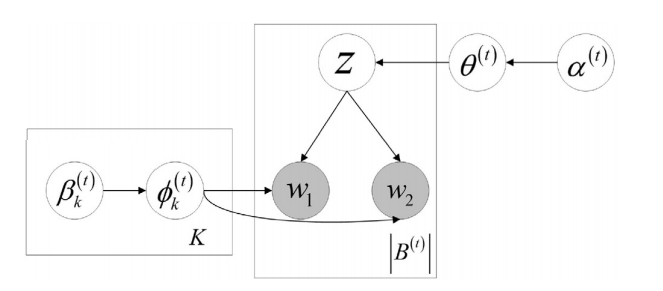
\includegraphics[width=10cm]{./figs/btm.png}
  \caption{$t^{th}$时间片内的BTM主题模型}
  \label{fig:btm}
\end{figure}

其中,K表示主题数,$B^{t}$表示由$\{w_1,w_2\}$组成的词对集合,称作一个biterm。
$\alpha^{(t)}$和$\beta_{k}^{(t)}$分别是 $\varphi^{(t)}$和$\theta^{(t)}$的Dirichlet分布的先
验参数,$\theta^{(t)}$是K维的文档-主题多项式分布,$\varphi^{(t)}$是W维的主题-词分布; $Z_{m,n}$表示词语的主题分布,$w_1$和$w_2$是在该分布下取样生成的词;
下面是BTM模型的生成步骤:
 
\begin{center}
  \begin{itemize}
\item Draw a topic distribution in the $t^{th}$ time slice $\theta^{(t)}~Dirichlet(\alpha^{(t)})$;
\item For each topic k from K topics:\\
        (a) Draw a word distribution of topic in the $t^{th}$ time slice $\varphi^{(t)}~Dirichlet(\beta^{(t)})$
      \item For each biterm $b_j = {w_{j,1},w_{j,2}} \in B^{(t)}$:\\
        (a) Draw a topic $z_j ~ Multinomial(\theta^{(t)})$;\\
        (b) Draw words $w_{j,1},w_{j,2} ~ Multinomial(\varphi_{z_{j}}^{(t)})$;\\
 \end{itemize}
\end{center}

由于短文本是以流的形式传入模型的,本文将流数据按时间顺序进行分块,并设置好块大小。每当数据块来临的时候,即使用BTM算法对块数据进行特征表示,得到块的特征值。本文实验数据总文本数为10000,共5个类别,采用的块大小为1000,BTM主题模型主题数为5,BTM迭代次数100次,借助python第三方库“biterm”,对BTM算法进行了调用,从而得到每个块的特征值。借助BTM模型,对扩展后的数据块$D_i^{'}$进行主题推断,将起表示为一组主题分布,即得到$D_i^{''}=\{d_j^{''}\}_{j=1}^{|D_i|}$,其中$d_j^{''}=\{z_{j,k}\}_{k=1}^K$,,$z_{j,k}$表示$j^{th}$短文本中$k^{th}$主题值。

\begin{table}[htb]
  \begin{singlespace}                                                          
    \centering\caption{BTM主题词提取结果}\label{tab:before}
    \renewcommand{\arraystretch}{1.5} %控制行高
    \begin{tabular}{l}\hline
Topic 0 | Top words = black friday chelsea mobile obama arsen \\
Topic 1 | Top words = obama presid bush czar blackberri smartphone \\
Topic 2 | Top words = chelsea arsen phone intern free obama \\
Topic 3 | Top words = win day smartphon chelsea tablet liverpool \\ 
Topic 4 | Top words = tangan jam murah hdmi ic 20 \\ 
\hline                                                      
     \end{tabular}                                                              
  \end{singlespace}
\end{table}               

% 我们使用Gibbs采样的方法,获得每个时间片$t^{th}$的文档-主题分布
% $\theta{(t)}=\{\theta_k^{(t)}\}_{k=1}^{K}$和主题-词分布
% $\varphi{(t)}=\{\varphi_k^{(t)}\}_{k=1}^{K}$,其中
% $\varphi_{k}=\{\varphi_{k|w}^{t}\}_{w=1}^{W}$。若每个短文本d中可生成$N_b$个无序词对,即
% $\{b_j^{d}\}_{j=1}^{N_b}$,其中$b_j^{(d)}=(w_{j,1}^{(d)},w_{j,2}^{(d)})$,则短文本的主题
% 为k的概率可以表示为:

% % \ref{eq:pkd}:

% \begin{equation}
%   \label{eq:pkd}
%  P(k|d) = \sum_{j=1}^{N_b} P(k|b_j^{(d)})P(b_j^{(d)}|d) 
% \end{equation}

% 其中,$P(k | b_j^{(d)})$表示短文本d中第j个词对是主题k的概率,$P(b_j^{(d)} | d)$表示短文本d中包
% 含词对$b_j^{(d)}$的概率。

% \subsection{主题跟踪}

\section{概念漂移检测}
在短文本数据流分类中,主题随着时间的推移发生会变化从而产生概念漂移。概念漂移会严重影响
到模型的预测精度,因此解决该问题对本模型十分重要。本文通过主题的分布
来检测检测概念漂移。


每当新的数据块来的时候,我们通过计算该数据块中的每个短文本和当前数据块的语义距离,再计算均
值来判断新数据块是否发生了概念漂移,公式\ref{eq:dist1}如下:

\begin{equation}
  \label{eq:dist1}
       dist(D_{i+1}^{''},D_{i}^{''})=1 / |D_{i+1}|\sum_{j=1}^{|D_{i+1}|}dist(d_j^{''},D_i^{''})
\end{equation}

其中,$dist(d_j^{''},D_i^{''})$为短文本和当前数据块之间的距离,首先根据类分布,将当前数据
块分割成大小为C的簇,记作$\{I_c\}_{c=1}^{C}$,其中$I_c=\{d_i^{''}\}_{I=1}^{|I_c|}$,
$|I_c|$表示$c^{th}$类簇中的短文本数,再计算短文本和所有类簇之间的语义距离,选择语义
距离最小的值表示该短文本与数据块之间的语义距离,如公式\ref{eq:dist2}:

\begin{equation}
  \label{eq:dist2}
  dist(d_j^{''}, D_i^{''})=min dist(d_j^{''},I_c)
\end{equation}

其中,$dist(d_j^{''},I_c)=1/|I_c|\sum_i^{|I_c|}dist(d_j^{''},d_l^{''}), d_I^{''} \in I_c $。图\ref{fig:concept-drift}是本算法的流程图。

\begin{figure}[H]
  \centering
  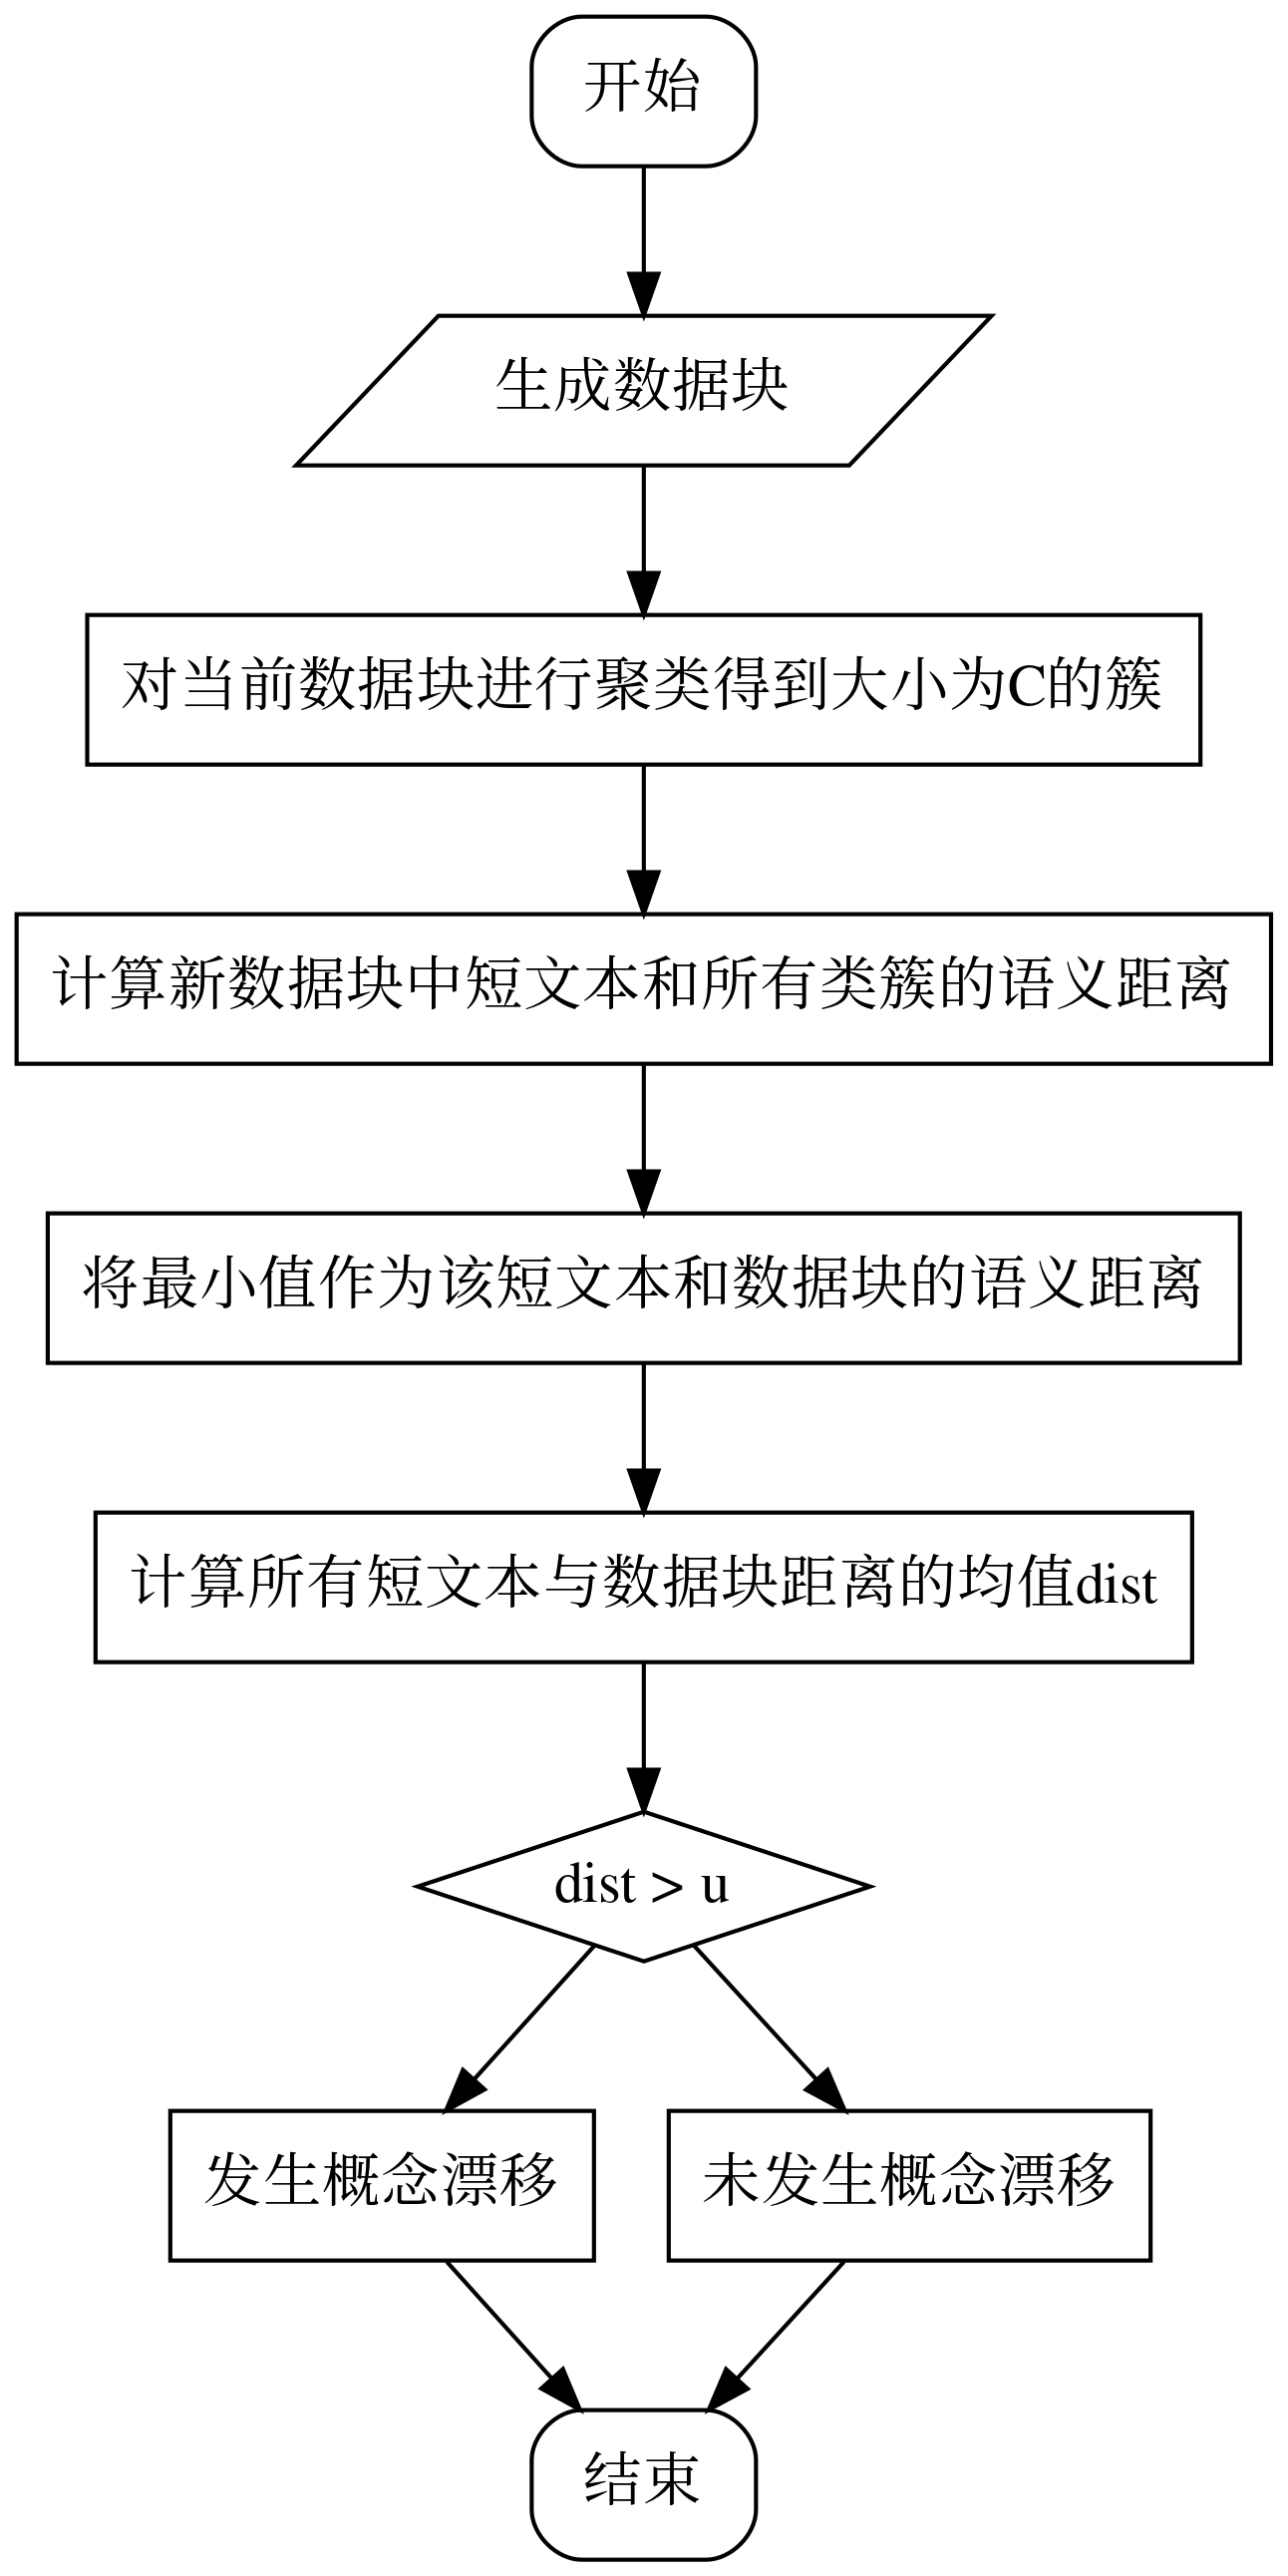
\includegraphics[width=0.4\textwidth]{concept-drift}
  \caption{概念漂移检测流程图}
  \label{fig:concept-drift}
\end{figure}

若某个类簇中的短文本数量很少,在计算两个短文本之间的语义距离$dist(d_j^{''},d_l^{''})$时便
会产生误差,由此对该项增加权重,如公式\ref{eq:dist3}:
\begin{equation}
  \label{eq:dist3}
   dist(d_j^{''},d_l^{''})=1-|I_c|/|D_i^{''}|cos(d_j^{''},d_l^{''})
 \end{equation}
 
其中,$cos(d_j^{''},d_l^{''})$为文本的余弦距离。

% \begin{equation}
%   \label{eq:cos}
% cos(d_j^{''},d_l^{''})=(z_{j,1}\cdot z_{l,1}+…+z_{j,K} \cdot
% z_{l,K})/\sqrt(\sum_{k=1}^{K}(z_{j,k})^2) \cdot\sqrt( \sum_{k=1}^{K}(z_{l,k})^2 )
% \end{equation}

最后,根据阈值u去判断是否发生概念漂移。如果$dist(D_{i+1}^{''},D_i^{''}) \in (u,1]$,则
认为数据块$D_{(i+1)}^{''}$发生了概念漂移。

\section{集成模型的构建与更新}
本章是算法的核心,构建并更新集成模型,用于预测未知标签的短文本数据。选择H个上述的数据块用于
构建SVM基分类器。当新的块$D_e$到来时,首先对它进行文本扩展和特征表示,然后使用BTM主题模型将其表示为一组主
题$D_e^{''}$。构建集成模型之前,要计算短文本$d_j^{''}$相对基
分类器的${f_h}$的权值$w_{h,j}$:

\begin{equation}
  \label{eq:w}
W_{h,j}  = (1-dist(d_j^{''},D_h^{''})) * (1-dist(D_e^{''}, D_h^{''}))
\end{equation}

其中,$1-dist(d_j^{''},D_h^{''})$表示数据块$D_e^{''}$和短文本$d_j^{''}$数据块$D_h^{''}$的语义相似度,$1-dist(D_e^{''},D_h^{''})$表示新数据块$D_e^{''}$和当前数据块$D_h^{''}$之间的语义相似度,用于减少概念漂移对准确率的影响。

下面是更新集成模型E的步骤,首先计算新数据块$D_e^{''}$和集成模型中每个旧数据块之间的语义距
离,并将新数据块构建一个分类器$f$。如果数据块$D_e^{''}$相对于E中的每个分类器都发生了概念漂
移,并且E中基分类器数量未满(即小于H),则将f添加到集成模型E中,如果E中基分类器数量已满,
则替换E中最老的基分类器。否则,将分类器f替换E中与其语义距离最小的基分类器。

% \begin{algorithm}[H]
% 	\renewcommand{\algorithmicrequire}{\textbf{输入:}}
% 	\renewcommand{\algorithmicensure}{\textbf{输出:}}
% 	\caption{集成模型更新与构建}
% 	\label{alg:ensemble}
% 	\begin{algorithmic}[1]
% 		\REQUIRE 文本数据 D,数据块 $D_e$,LDA 主题模型 $M_{LDA}$,BTM主题模型$M_{BTM}$,集成模型 E, 数
%         据块大小 H
% 		\ENSURE 数据流 S, 概念漂移检测阈值 $\mu$
% 		\STATE 利用$M_{LDA}$进行语义扩展,将$D_e$扩展为$D_e^{'}$
% 		\STATE 利用$M_{BTM}$进行特征表示,将$D_e^{'}$ 表示为 $D_e^{''}$
%         \FOR{$D_h^{''}$ in S}
%         \STATE 计算新数据块$D_e^{''}$和$D_h^{''}$的语义距离
%         \STATE 将新数据块$D_e^{''}$构建一个SVM分类器$f_e$
% 		\ENDFOR
%         \IF {数据块$D_e^{''}$相对于E中的每个分类器都发生了概念漂
%           移 \textbf{and} E中基分类器数量 < H}
%         \STATE 将f添加到集成模型E中
%         \ENDIF
%   \end{algorithmic}  
% \end{algorithm}

  \begin{algorithm}[H]
	\renewcommand{\algorithmicrequire}{\textbf{输入:}}
	\renewcommand{\algorithmicensure}{\textbf{输出:}}
	\caption{集成模型更新与构建}
	\label{alg:ensemble}
	\begin{algorithmic}[1]

		\REQUIRE 未到达数据块 D,LDA 主题模型 $M_{LDA}$,BTM主题模型$M_{BTM}$
		\ENSURE 数据流 S,集成模型 E,概念漂移检测阈值 $\mu$
		\FOR{$D_e$ in D}
		\STATE 利用$M_{LDA}$进行语义扩展,将$D_e$扩展为$D_e^{'}$
		\STATE 利用$M_{BTM}$进行特征表示,将$D_e^{'}$ 表示为 $D_e^{''}$
        \FOR{$D_h^{''}$ in $S$}
         \FOR{$d_j^{''}$ in $D_e^{''}$}
        \STATE  计算短文本 $d_j^{''}$ 和旧数据块 $D_h^{''}$ 的语义距离(公式\ref{eq:dist2})
        \ENDFOR
        \STATE 计算新数据块$D_e^{''}$ 和 旧数据块$D_h^{''}$ 的语义距离(公式\ref{eq:dist1})
         \ENDFOR
          \FOR{$d_j^{''}$ in $D_e^{''}$}
          \STATE 计算基分类器权重(公式\ref{eq:w})          
          \STATE  使用集成模型预测新数据块中的短文本 $d_j^{''}$ (公式\ref{eq:predict})
          \ENDFOR
          \STATE 计算$D_e^{''}$ 和 S 中每个块的语义距离,并根据阈值$u$判断是否发生了概念漂移
          \STATE 使用数据块 $D_e^{''}$ 训练新的基分类器$f$,并根据概念漂移的结果更新集成模型
		\ENDFOR
	\end{algorithmic}  
  \end{algorithm}


% \begin{algorithm}[H]
% 	\renewcommand{\algorithmicrequire}{\textbf{输入:}}
% 	\renewcommand{\algorithmicensure}{\textbf{输出:}}
% 	\caption{集成模型更新与构建}
% 	\label{alg:ensemble}
% 	\begin{algorithmic}[1]

% 		\REQUIRE 文本数据 D,数据块 $D_e$,LDA 主题模型 $M_{LDA}$,BTM主题模型$M_{BTM}$,集成模型 E, 数
%         据块大小 H
% 		\ENSURE 数据流 S, 概念漂移检测阈值 $\mu$
% 		\FOR{$D_e$ in D}
% 		\STATE 利用$M_{LDA}$进行语义扩展,将$D_e$扩展为$D_e^{'}$
% 		\STATE 利用$M_{BTM}$进行特征表示,将$D_e^{'}$ 表示为 $D_e^{''}$
%         \FOR{$D_h^{''}$ in $S$}
%          \FOR{$d_j^{''}$ in $D_e^{''}$}
%         \STATE  使用公式\ref{eq:dist2}计算 $d_j^{''}$ 和 $D_h^{''}$ 的语义距离
%         \ENDFOR
%         \STATE 使用公式\ref{eq:dist1}计算 $D_e^{''}$ 和$D_h^{''}$ 的语义距离
%          \ENDFOR
%           \FOR{$d_j^{''}$ in $D_e^{''}$}
%           \STATE 使用公式\ref{eq:w}计算基分类器权重          
%           \STATE  使用集成模型预测 $d_j^{''}$ 
%           \ENDFOR
%           \STATE 计算$D_e^{''}$ 和 S 中每个块的语义距离,并根据阈值$u$判断是否发生了概念漂移
%           \STATE 使用数据块 $D_e^{''}$ 训练新的基分类器$f$,并根据概念漂移的结果更新集成模型
% 		\ENDFOR
% 	\end{algorithmic}  
%   \end{algorithm}

% \begin{algorithm}
% 	\renewcommand{\algorithmicrequire}{\textbf{Input:}}
% 	\renewcommand{\algorithmicensure}{\textbf{Output:}}
% 	\caption{Ensemble Algorithm}
% 	\label{alg:1}
% 	\begin{algorithmic}[1]
% 		\REQUIRE String data D, the LDA topic model $M_{LDA}$, the ensemble model E, the set of H data;
% 		\ENSURE chunks used for the ensemble model S, the threshold $\mu$;
% 		\FOR{each data chunk $D_e$ in D}
% 		\STATE Expand $D_e$ with the topic model $M_{LDA}$ as $D_e^{'}$;
% 		\STATE Represent expaned $D_e^{'}$ as $D_e^{''}$ using BTM;
%         \FOR{$D_i^{''}$ in $S$}
%          \FOR{$d_i^{''}$ in $D_e^{''}$}
%         \STATE  Calculate semantic distance between $d_j^{''}$ and $D_i^{''}$ using \ref{eq:dist2}
%         \ENDFOR
%         \STATE Calculate semantic distance between $D_e^{''}$ and $D_i^{''}$ using \ref{eq:dist1}
%          \ENDFOR
%           \FOR{$d_i^{''}$ in $D_e^{''}$}
%           \STATE Calculate weights using \ref{eq:w}
%           \STATE  Predict $d_j^{''}$ according to ensemble model E using \ref{eq:1}
%           \ENDFOR
%           \STATE Detect concept drifts between $D_e^{''}$ and each data chunk in S
%           according to the threshold $\mu$;
%           \STATE Build a new classifier $f$ on $D_e^{''}$ and update ensemble model E according to results of concept drifts;
% 		\ENDFOR
% 	\end{algorithmic}  
%   \end{algorithm}

  
% \begin{algorithm}
% \caption{Ensemble Algorithm}
% \hspace*{0.02in} {\bf Input:} %算法的输入,
% % String data D, the LDA topic model $M_{LDA}$, the ensemble model E, the set of H data
% % \\
% \hspace*{0.02in} {\bf Output:} %算法的结果输出
% %updated E, predicted lables in data chunk $D_e$;
% \label{alg:Ensemble}
% \begin{algorithmic}

% % \For{} % For 语句,需要和EndFor对应
% % 
% %\EndFor
% \end{algorithmic}
% \end{algorithm}

% \section{实验结果和分析}

% \subsection{实验数据和评价指标}

% \subsection{基准方法和参数设置}

% \subsection{性能分析}

\section{本章小结}
本章主要介绍了本文核心算法的技术细节,提出一种带漂移检测的短文本分类算法,给出了算法的数学推导以
及运作流程。首先说明了数据集的来源,给出了短文本数据流分类的问题定义。通过Wikipedia将短文
本数据进行扩展并用BTM模型表示成主题,将数据流分块形成多个基分类器,构建集成模型,并进行了概念漂移的检
测,得到一个可用的集成分类模型,用于新数据的预测。

